

\documentclass[12pt]{article}
%\documentclass[10.8pt, a4paper, USenglish, twocolumn]{article}

\usepackage{isaks_template} % Contains all included packages. See isaks_template.sty.

% latex margins
\linespread{1.5}
\newgeometry{vmargin={15mm}, hmargin={25mm,37mm}}
%
\title{Project Thesis\\ Solving Biharmonic Equation using \\ Continuous Interior Penalty Method}
\author{Isak Hammer }
\date{\today}

\begin{document}
    \begin{titlepage}
        \maketitle
        \begin{figure}
        \centering
        % 
\includegraphics[width=0.5\textwidth]{figures/front_page/dog.jpg}\\
        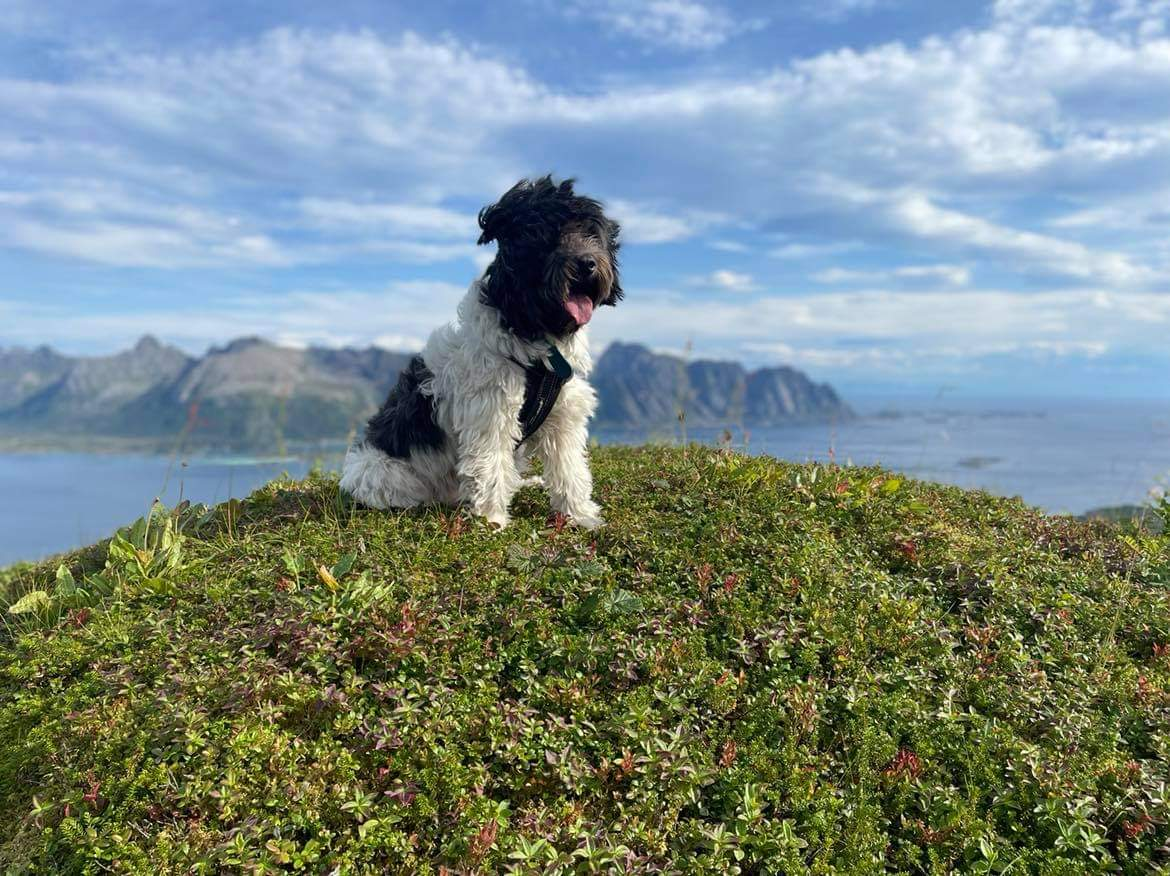
\includegraphics[width=0.5\textwidth]{figures/front_page/molly.jpeg}\\
        \end{figure}
        \thispagestyle{empty}
    \end{titlepage}

    \newpage
    \label{sec:eyyy}


    \section{Introduction}\label{sec:introduction}


The biharmonic equation is a fourth order partial differential equation which has gained great importance in
application such as mathematical modelling of linear elastic theory \cite{selvadurai13} and phase separation mechanics
of two phase systems \cite{cahnhilliard1957, kim16}. However, methods for solving the biharmonic equation analytically
is considered extensive and often impossible. Even on very simple plane problems on a unit square often requires advanced computations using integral transforms, variable separations, complex analysis and more \cite{selvadurai13}. We therefore tend
to lean towards approximating the solution using numerical methods for complicated problems.

There is generally two classes of numerical methods to solve the biharmonic equation. The first class is known as finite difference method (FDM) \cite{geer06,ehrlich75, hackbusch17}. Nevertheless, FDM does not handle complex domains well since it generally has strict requirements for the mesh generation. However, some methods have been introduced to solve problems on irregular domains, but is has shown to be relative extensive to implement \cite{hackbusch17, chen08, belyaev18}.

The second class is denotes as finite element method (FEM). Using this methods implies that there is theoretically no difference on solving problems on a regular or irregular domains, except for taking account for numerical stability and some
restrictions on mesh generation \cite{chen08}. However, a major challenge in FEM is to choose a discrete solution space on the finite elements to approximate the exact solution. We say that a method is conforming if the discrete solution space
$V_{h}$ is subspace of the exact solution space $V$, i.e. $V_{h} \subseteq  V$ \cite{shi02, brenner07math}. In general, for conforming methods requires that for a problem of order $2n$ must the discrete solution space be at least of order $n-1$. Thus, for a biharmonic problem
will a conforming FEM method demand at least a basis that is $C^1$ globally \cite{shi02}. From this strong continuity conditions rises a lot of complexity when constructing a finite element. In fact, attempts to solve this problems has shown that it
arise 21 degrees of freedom in a triangular Argyris element \cite{nair21}.

For nonconforming methods, $V_{h} \not \subseteq  V_{h}$ is the $C^{1}$ requirement completely relaxed. This makes the methods more suitable for forth order problems with the cost of more extensive error analysis. In fact, designing nonconformal
elements that does converge is rather difficult \cite{shi02, nair21}.

A third approach of FEM to solve the biharmonic equation is to solve the problem doing a mixed FEM method. This method seems promising, because it only requires $C^{0}$ elements \cite{chen08, brezzi91}.
Though this work well from a numerical point of view it has shown to have drawbacks by replacing symmetric positive definite continuous problem
by a saddle point problem, which is certainly makes the existence and uniqueness proof more challenging \cite{brezzi74}.

In this report will we focus to work on a fourth approach known as the continuous interior penalty method (CP). A major advantage is that the approach preserves the global $C^{0}$ continuity and the positive symmetric definiteness, thus makes it attractive to solve the biharmonic equation \cite{brenner2012, brenner2012quadratic}. In this report will we focus on presenting the derivation of CP and carry out a basic error analysis. We will also present a numerical analysis.


\section{Mathematical Background}%
\label{sub:mathematical_background}

In this section will we briefly establish some basic results of functional analysis and numerical analysis in order to construct the foundations of the FEM method. However, for a more thoroughly explanation some recommended sources are
\cite{brenner07math,manzoni2021optimal, quartdiff}. We will first define basic principles of Hilbert spaces which then will be applied to establish a theory for weak formulations the notion of a well-posed problem. Moreover, we will then continue by
establishing error estimates and constructing a numerical discretization of the weak formulation using a simple test problem.

\subsection{Hilbert Spaces}%
\label{sub:hilbert_spaces}

Assume $\Omega $  to be a compact and open set in $\mathbb{R} ^{2}$ and the parameter $p \in \mathbb{R} $, $p\ge 1$. We define $L^{p}\left( \Omega  \right) $ to be the set of all measurable functions $f: \Omega  \mapsto \mathbb{R} $ such that
$\left\lvert f \right\rvert ^{p}$ is Lebesgue measurable, i.e,

\begin{equation*}
    L^{p}\left( \Omega  \right) = \left\{ f: \Omega \mapsto \mathbb{R}  \mid \int_{\Omega }^{} \left\lvert f \right\rvert ^{p} d \Omega  < \infty  \right\}
.\end{equation*}

A useful extension which we will use later are the set of locally integrable functions such that for any compact subset $K \subseteq \text{Interior}\left( \Omega  \right) $, that is

\begin{equation*}
    L_{loc}^{1}\left( \Omega  \right)  = \left\{ f: f \in L^{1}\left( \Omega  \right)  \quad \forall K  \right\}.
.\end{equation*}


Let $u \in L^{p}\left( \Omega  \right) $, then we define the integral norm of order $p$ to be \[
\| u \|_{ L^{p}\left( \Omega  \right)  }^{  }  = \left( \int_{\Omega }^{} \left\lvert u \right\rvert ^{p} dx  \right) ^{\frac{1}{p}}
\]

Since $p=2$ is very frequently used we also define a more compact notation $\| u \|_{ \Omega  }^{  }  = \| u \|_{ L^{2}\left( \Omega  \right)  }^{  } $ .  We say that $L^{2}\left( \Omega  \right) $ is a Hilbert space if it is equipped with a inner
product of two functions $u,v \in L^{2}\left( \Omega  \right) $ such that
\[
\left( u,v \right) _{\Omega } = \left( u,v \right) _{L^2\left( \Omega  \right) } = \int_{\Omega }^{} u \cdot v dx
\]

In this report will we use the notation $\mathcal{V} $ for arbitrary Hilbert space. Note that we also use the notation $V^{*}$ for the dual space.

We will now establish a nation of the weak derivative, but first are we going to characterize some useful definitions of continuity. The space $C^{k}\left( \Omega  \right) $ for $k\ge 0$ denotes the set of functions whose derivatives, up to order of
$k$ , is continuous in $\Omega $. Note that we often use the shorthand notation \[
C^{0} = C\left( \Omega  \right)  = C^{0}\left( \Omega  \right)
\]
From this definitions we let $C^{\infty}\left( \Omega  \right) $ be the set of infinitely differentiable functions in $\Omega $ such that the space $C^{\infty}_{0}\left( \Omega  \right)$ is the set of all functions $u \in C^{\infty}\left( \Omega
\right) $ which is vanishing outside of any compact subset of $\Omega $. Let $u,v \in  C^{1}\left( \Omega  \right) $ and $\Gamma  = \partial \Omega $ with corresponding outer normal vector $n$, then this partial integration formula holds

\[
\int_{\Omega }^{} \nabla u \cdot v dx = \int_{\Gamma }^{} u\cdot v n ds - \int_{\Omega }^{} u \cdot \nabla v dx
\]

We now use this notation for derivatives \footnote{In literature is often $D^{\alpha } f$ commonly used, but later in the report is this notation reserved for the Hessian operator. }, $f \in C^{\left\lvert \alpha  \right\rvert } \left( \Omega  \right) $ so \[
\partial _{\alpha  } f = \frac{\partial ^{\left\lvert \alpha  \right\rvert } f}{ \partial ^{\alpha _{1} } x_{1} \partial ^{\alpha _{2}} x_{2}  }, \quad \alpha=\left( \alpha _{1}, \alpha _{2} \right)
\]


Finally, let $u \in  L^{1}_{loc}\left( \Omega  \right) $. We call the function $w \in L_{loc}^{1}\left( \Omega  \right) $ the $\alpha $-th weak derivative of $u$  if \[
\int_{\Omega }^{} w \varphi  dx = \left( -1 \right) ^{\left\lvert \alpha  \right\rvert } \int_{\Omega }^{} u \cdot \partial _{\alpha } \varphi dx, \quad \forall \varphi \in  C_{0}^{\infty}\left( \Omega  \right)
\]

Using the definitions introduced in this subsection can we construct the Sobolev space $H^{m}\left( \Omega  \right) , m>1$ , \[
H^{m}\left( \Omega  \right) = \left\{ u \in L^{2}\left( \Omega  \right)  \mid  \partial _{\alpha } u \in L^{2}\left( \Omega  \right)  \forall \alpha : \left\lvert \alpha  \right\rvert  \le m \right\}
\]

Equipped with the inner product is $H^{m}\left( \Omega  \right) $  denoted as a Hilbert space, that is, for $u,v \in H^{m}\left( \Omega  \right) $ is \[
    \left( u,v \right) _{H^{m}\left( \Omega   \right) } = \sum_{\left\lvert \alpha  \right\rvert  \le  m}^{}  \int_{\Omega }^{} \partial _{\alpha } u \partial _{\alpha } v dx.
\]

Similarly the integral norm is \[
\| u \|_{ H^{m}\left( \Omega  \right)  }^{  }  = \left( \| u \|_{ L^{2}\left( \Omega  \right)  + \sum_{k = 1}^{m}  \left\lvert u \right\rvert ^{2}  }^{  H^{k}\left( \Omega  \right) }  \right) ^{\frac{1}{2}}
\]
where the seminorm is define such that \[
\left\lvert u \right\rvert _{H^{k}\left( \Omega  \right) } = \left( \sum_{\left\lvert \alpha  \right\rvert  = k}^{} \| \partial _{\alpha }u \|_{ \Omega  }^{ 2 }  \right).
\]

We may also entitle the notation $H^{m}_{0} \left( \Omega  \right) = H^{m} \left( \Omega  \right) \cap C^{\infty}_{0} \left( \Omega  \right) $.





\subsection{Weak Formulation}%
\label{sub:weak_formulation}

By applying the theory in the previous subsection can we use describe the notion of a so-called weak formulation. Let us consider the simplest case, that is the strong form of the Poisson's equation with homogeneous Dirichlet boundary conditions
\begin{equation}
\label{eq:poisson_strong}
\begin{split}
-\Delta u & = f \quad \text{in } \Omega \\
u & =0 \quad \text{on } \partial \Omega
\end{split}
.\end{equation}

We want to obtain the weak formulation of the problem \eqref{eq:poisson_strong}. Let the trial function be $u \in H_{0}^{1}\left( \Omega  \right) $, then by integrating with a test function we get \[
\int_{\Omega }^{} - \Delta u \cdot v dx = \int_{\Omega }^{} f \cdot v dx \quad \forall v \in H^{1}_{0}\left( \Omega  \right)
\]
By using the partial integration formula and take the advantage of homogeneous Dirichlet boundary conditions the equation is in fact simplified to \[
a\left( u,v \right) = \int_{\Omega }^{}  \nabla u\cdot \nabla v dx , \quad l\left( v \right)  = \int_{\Omega }^{}  f\cdot v dx
\]

Hence, the final weak formulation has a symmetric bilinear form, $a\left( \cdot ,\cdot  \right) $, and a linear functional, $l\left( \cdot  \right) $, where we want to find a solution $u \in H^{1}_{0}\left( \Omega  \right) $  so

\begin{equation}
\label{eq:poissons_weak_formulation}
a\left( u,v \right) = l\left( v \right) \quad \forall v \in H^{1}_{0}\left( \Omega  \right).
.\end{equation}

We now want to establish that problems on this form is well-posed.
Lax-Milgram Theorem says that if we assume a Hilbert space $\mathcal{V} $ and the bilinear symmetric problem where we want to find a $u \in \mathcal{V} $  such that

\begin{equation*}
    a\left( u,v \right)  = \left( F, v \right) _{\mathcal{V} ^{*}, \mathcal{V} }, \quad \forall v \in  \mathcal{V}
.\end{equation*}

 Assuming the bilinear form $a\left( \cdot ,\cdot  \right) $  is continuous and coercive, i.e., the two conditions below.

\begin{enumerate}[label=\arabic*)]
    \item There exists a constant $M>0$ s.t. \[
    \left\lvert a\left( v,w \right)  \right\rvert \le M \| v \|_{ \mathcal{V}  }^{  } \| w \|_{ \mathcal{V}  }^{  }  \quad \forall v,w \in \mathcal{V}.
    \]
\item There exists a $\alpha  > 0$  so \[
a\left( v,v \right)  \ge  \alpha \| v \|_{ \mathcal{V}  }^{ 2 }.
\]
\end{enumerate}

We can then say there exists a unique solution $u \in \mathcal{V} $ and in additions it satisfied the stability estimate \cite{manzoni2021optimal}, \[
\| w \|_{ \mathcal{V}   }^{  } \le  \| F \|_{ V^{*} }^{  }
\]
Problems that fulfills this criteria is said to be well posed.


We can clearly see that this theorem applied to the weak formulation \eqref{eq:poissons_weak_formulation} since,
\[
\begin{split}
    \left\lvert a\left( v,w \right)  \right\rvert & \le \| \nabla v \|_{ \Omega  }^{  } \| \nabla w \|_{ \Omega  }^{  }, \\
\left\lvert a\left( v,v \right)  \right\rvert  & = \|  \nabla v\|_{\Omega   }^{  }  \| \nabla v  \|_{\Omega   }^{  } \ge  \| v \|_{ \Omega  }^{ 2 } \ge \| v \|_{ H^{1}\left( \Omega  \right)  }^{  }.
\end{split}
\]

On the last inequality was the Poincare inequality applied, i.e., there exists a $C>0$  such that $\| u \|_{ \Omega  }^{  } \le C  \| \nabla u \|_{\Omega   }^{  } $.


\subsection{Ceas' Lemma}%
\label{sub:ceas_lemma}

Since we have established a theory of a well-posed weak formulation we can now transition to setup a theory for a approximate solution. Assume that we have a problem that satisfied the Lax-Milgram theorem and let $\mathcal{V} _{h} \subseteq  \mathcal{V} $  be
some finite dimensional subspace of $\mathcal{V} $ such that $dim\left( \mathcal{V} _{h} \right) =N_{h}$ , where $h$  is a discretization parameter. The discretized problem is now to find a solution $u_{h} \in  \mathcal{V}_{h}$ such that $a\left( u_{h},v_{h} \right)  =
l\left( v_{h} \right) \quad  \forall v_{h} \in \mathcal{V} _{h} $. In fact, since the method is conform, i.e., $\mathcal{V} _{h} \subseteq  \mathcal{V} $ does it exists a exact solution $u \in  \mathcal{V} _{h}$ so, \[
a \left( u, v_{h} \right)  = l\left( v_{h} \right)  \quad  \forall v_{h} \in  \mathcal{V} _{h}.
\]

Using property can  we say that the problem is strongly consistent since it fulfills the Galerkin Orthogonality property, that is,  $ a\left( u -u_{h} , v_{h} \right)  =0$.

Now we have all the cornerstones for finding a error estimate . Again, assume that Lax-Milgram theorem holds. Let $v_{h} \in  \mathcal{V} _{h}$ so
\[
    \begin{split}
\alpha \| u -u_{h} \|_{ \mathcal{V}  }^{ 2 } & \le  a\left( u - u_{h}, u - u_{h}  \right)    \\
&= a\left( u - u_{h}, u -v_{h} \right) - a\left( u -u_{h}, v_{h} - u_{h} \right)  \\
\le  M \| u - u_{h} \|_{ \mathcal{V}  }^{  }  \| u - v_{h} \|_{ \mathcal{V}  }^{  }
    \end{split}
\]
Hence, the Ceas' lemma \cite{quartdiff} \[
\| u - u_{h} \|_{ \mathcal{V}  }^{  }  \le  \frac{M}{\alpha } \inf_{v_{h} \in \mathcal{V} } \|  v_{h} - u \|_{  }^{  }
\]

A useful property is that for a conformal numerical method to converge can we now only require \[
\lim_{h \to 0}  \inf_{v_{h} \in  V_{h}}  \| v - v_{h} \|_{ \mathcal{V }  }^{  } = 0 \quad  \forall v \in \mathcal{V}.
\]

In that case will $\| u - u_{h} \|_{ \mathcal{V}  }^{  }  \to  0$, $h \to  0$ .



\subsection{Finite Element Method}%
\label{sub:finite_element_method}
The idea of a conformal FEM method is to approximate a solution $\mathcal{V}_h \subseteq \mathcal{V}  $. However, the build blocks of the discretization relies on constructing a trianguation $\mathcal{T } _h$ with non-overlapping triangles  $T \in
\mathcal{T}_{h} $ so that \[
\Omega _{h} = Interior(\bigcup_{T \in  \mathcal{T} _{h}}^{} T) \implies \lim_{h\to 0} measure(\Omega - \Omega _{h}) = 0 \text{ a.e.}.
\]

For convenience will we generally use the notation $\Omega  = \Omega  _{h}$. We also denote the parameter $h$ as the diameter of the triangle $T$, i.e., $h_{T} = diam(T)$. Anyhow, this is later more precisely in the subsection
\ref{sub:computational_domain} later on, but for now does it hold as a basic introduction to conformal FEM.
Furthermore, let the space of finite elements suitable for our test problem in subsection \ref{sub:weak_formulation}, using the definition from \cite{quartdiff}, to be
\[
\mathcal{V} _{h} = \left\{ v_{h} \in C^{0}\left( \Omega  \right)  \mid  v_{h} \in \mathcal{P} _{r}\left( T \right)  \quad \forall T \in \mathcal{T} _{h}  \right\}
\]
where $\mathcal{P } _{r}\left( T \right) $ is the space of polynomials with degree $r$ for each $T$, that is,
\[
\mathcal{P} _{r}\left( T \right)  = \left\{ p\left( x_{1}, x_{2} \right) = \sum_{}^{i + j}  a_{ij} x^{i}_{1} x^{j}_{2}  \mid  a_{ij} \in \mathbb{R}  \text{ and } i,j \ge  0   \right\}.
\]

For the test problem can we observe that it is convenient to deal with a Lagrangian functions $\varphi _{j} \in V_{h}$, thus, for ever node $N_{u}$, \[
\varphi _{j}\left( N_{i} \right)  = \delta _{ij} = \begin{cases}
    0, \quad & i \neq j \\
    1,\quad & i=j
\end{cases}
\text{ where } i,j = 1,\ldots, N_{h}.
\]

Here is $N_{h}$  the total number of nodes which is chosen with caution. For the test problem, where $\Omega \subseteq \mathbb{R} ^{2} $, when $r=1$ is typically the nodes defined on the vertices and $ r=2 $ the nodes defined on the vertices and the
center of the edges/facets \cite{quartdiff}.
















    \newpage
\section{ Biharmonic Equation}
\label{sec:ch1}


Let $\Omega \subset   \mathbb{R} ^2$ be a bounded polygonal domain and $\partial \Omega $ be its corresponding boundary. Let the fourth order biharmonic equation have the form,

\begin{equation}
\label{eq:bi_problem}
\begin{split}
    \Delta^2  u  + \alpha  u  & = f \quad \text{in } \Omega   \\
    \partial _{n} u & = g_1\left( x \right)  \quad \text{on } \partial \Omega  \\
    \partial _{n} \nabla ^2 u & = g_{2}\left( x \right)  \quad \text{on } \partial \Omega .  \\
\end{split}
.\end{equation}
Here is $\Delta ^2$ the biharmonic operator, also known as the bilaplacian. We will assume for now that $u \in H^{4}\left( \Omega  \right) $, $\alpha $ is a nonnegative constant and $f \in L_{2}\left( \Omega  \right) $. We may consider the functions $g_{1}$ and $g_{2}$ as time independent boundary conditions. Such problems as \eqref{eq:bi_problem} are often associated with the Cahn-Hilliard model
\cite{cahnhilliard1957} for phase seperation. As a matter of fact, the major difference is that \eqref{eq:bi_problem}
has no time dependencie. However, depending on how Cahn-Hilliard model is time discretized numerically can
\eqref{eq:bi_problem} naturally arise. I refer to \cite{brenner2012quadratic} for more informastion on this.

Before we start constructing a numerical method, we might want to introduce the basic weak formulation of \eqref{eq:bi_problem}. Now, let the solution space be on the form,
\begin{equation*}
V = \left\{ v \in H^2\left( \Omega  \right) : \partial _{n} v = g_{1}  \text{ on }
\partial \Omega  \right\}.
.\end{equation*}
Consider the weak formulation to solve for a $u \in  V$ such that
\begin{equation}
    \label{eq:bi_weak1}
a\left( u,v \right)_{\Omega } = F(v).\quad \forall v \in
V,
\end{equation}
where the terms are computed as \[
    \begin{split}
a\left( u,v \right)_{\Omega } & = \int_{\Omega }^{} \left( D ^2 u : D ^2 v  +
\alpha  u v \right) dx , \\
F\left( v \right)_{\Omega } & = \left( f,v \right)_{\Omega } - \left<g_{2},v \right>_{\partial \Omega } + \left<\nabla g_{1}, \nabla v \right>_{\partial \Omega }.
    \end{split}
\]
We denote $D^2$ as the Hessian matrix operator. In fact, the solution is unique for $\alpha  > 0$. However, for $\alpha  = 0$ must we assume the solvability condtion,
\begin{equation*}
 \int_{\Omega }^{} f dx = \int_{\partial \Omega }^{} g_{2} ds
.\end{equation*}
This condition easily arise when using the substitution $v=1$ in \eqref{eq:bi_weak1}. To handle this, can we extended the solution space \[
V^{*} = \begin{cases}
    V \quad & \alpha  > 0 \\
    \left\{ v \in V: v\left( p_{*} \right)  = 0\right\}, \quad & \alpha  = 0
\end{cases}
\]
where $p_{*}$ is a corner of the polygonal domain $\Omega $.
Thus, the unique solution in $v \in V^{*}$ belongs to $H^{3 }\left( \Omega  \right) $ and we get the follwing
elliptic regularity estimate \cite{gu2012c0},
\begin{equation}
\label{eq:bi_harmonic_ellitpic_regularity}
\left| u \right| _{H^{3 }\left( \Omega  \right) }  \le C_{\Omega } \left( \| f \|_{  L_{2}( \Omega ) }^{  } + ( 1 + \alpha  ^{\frac{1}{2}}
) \cdot \| w  \|_{ H^{4}\left( \Omega  \right)  }^{  }    \right), \quad w\in H^{4}\left( \Omega  \right).
\end{equation}
This regularity estimate may be important for further usecases in terms of error analysis.


    \newpage
\section{Continious Interior Penalty Method}%
\label{sec:continious_interior_penalty_method}


To solve this numerically do we want to introduce the $C^{0}$ Interior Penalty Method (CP), which is a Discontinious Galerkin
method (DG) using $C^{0}$ finite elements. There is several reasons why we want to apply $C^{0}$ instead of the often used
$C^{1}$ finite elements for fourth order problems. First and foremost is the $C^0$ finite elements simpler than
obtaining $C^{1}$ finite elements.  Also, compared to other methods similar to the mixed
finite element method for the problem \eqref{eq:bi_problem}, CP has in fact
preserved the symmetric positive definiteness, which means the stability analysis is more straight forward. Finally and most
importantly according to \cite{brenner2012quadratic} can naive use mixed methods of splitting the boundary conditions of
the problem \eqref{eq:bi_problem} produce wrong solutions if $\Omega $ is nonconvex.

\begin{figure}[!h]
\centering
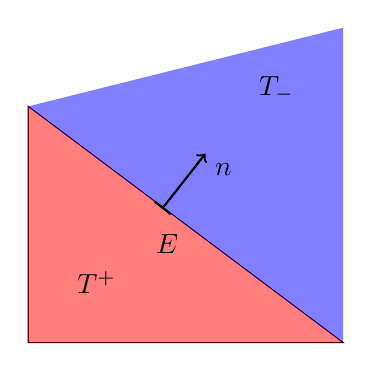
\begin{tikzpicture}[scale=1]
\coordinate (A) at (0,0);
\coordinate (C) at (0,3);
\coordinate (B) at (4,0);
\coordinate (D) at (4,4);
\coordinate (Tm) at (3.5,3.5);
\coordinate (Tp) at (0.5, 0.5);
\coordinate (e) at (1.5, 1.5);
\coordinate (start) at (1.7, 1.7);
\coordinate (end) at (2.25, 2.4);

\draw (A) -- (B) -- (C) -- cycle;
\fill[red, opacity=0.5] (A) -- (B) -- (C);
\fill[blue, opacity=0.5] (B) -- (C) -- (D);
\node[below left] at (Tm) {$T_{-} $ };
\node[above right] at (Tp) {$T^{+}$ };
\node[below right] at (e) {$E$ };

\draw [|->, thick] (start) -- (end);
% \node[above right] at (A) {A };
% \node[below right] at (B) {B};
% \node[above right] at (C) {C };
% \node[below right] at (D) {D};
\node[below right] at (end) {$n$};
\end{tikzpicture}
\caption{Edge $E \in \mathcal{F}_h $ shared by the triangles $T^{+}, T^{-} \in \mathcal{T}_{h} $ and the normal unit vector $n$.  }
    \label{fig:normal}
\end{figure}

Let $w,v \in  H^{4} \left( T  \right) $ and $\mathcal{T}_{h} $ the simplicial triangulation of $\Omega$. Using the same method as in \cite{gu2012c0, brenner2012quadratic} can we
deduce that for every triangle $T \in  \mathcal{T}_{h} $ is \[
    \begin{split}
        \left( \Delta  ^{2} w, v \right) _{T} &= \left< \partial _{n} \nabla ^2 w, v \right>_{\partial T} - \left( \nabla \left( \nabla ^2 w
 \right), \nabla  v  \right)_{T}   \\
 &= \left( D^2w, D^2v \right)_{T} + \left< \partial _{n} \nabla ^2 w, v \right>_{\partial T}  - \left<\partial _{n}
 \nabla w, \nabla v \right>_{\partial T} \\
 &=  \left( D^2 w, D^2 v \right)_{T} - \left<\partial _{nt} w, \partial _{t} v \right>_{\partial T} - \left<\partial
 _{nn} w, \partial _{n} v \right> _{\partial T} +  \left<\partial _{n} \nabla ^2 w, v \right>_{\partial T} \\
    \end{split}
\]
Keep in mind that this result naturally arise when defining $\nabla  = \left( \partial _{n}, \partial _{t} \right) $ such that
\[
\left<\partial _{n} \nabla w, \nabla v \right>_{\partial T} = \left<\partial _{nt} w, \partial _{t} v\right> _{\partial
T} + \left< \partial _{nn} w, \partial _{n} v  \right> _{\partial T} .
\]
 Thus, letting $u,v \in
H^{4}\left( T  \right) $  does this hold ,

\begin{equation}
\label{eq:bi_basic_dg}
\left( \Delta  ^{2} u,v \right) _{T} =  \left( D^2u,D^2v \right) _{T } - \left<\partial _{nt} u, \partial _{t}v
\right>_{\partial T} - \left<\partial _{nn} u, \partial _{n}v \right>_{\partial T} + \left<\partial _{n} \nabla ^2 u,v
\right>_{\partial T}
.\end{equation}

For global continuity, let  $v \in V =  \left\{ v \in H^{1}\left( \Omega  \right): v_{T} \in  H^{4}\left( T \right), \ \forall T \in
\mathcal{T}_{h}    \right\}   \cap C^{0} (
\overline{\Omega }  ) $ and $u \in  H^{4}\left( \Omega  \right) $ such that,

\begin{equation}
\label{eq:bi_basic_dg2}
\left( \Delta  ^{2} u,v \right) _{\Omega } = \sum_{T \in  \mathcal{T} _{h}}^{} \left( D^2u,D^2v \right) _{T } - \left<\partial _{nt} u, \partial _{t}v
\right>_{\partial T} - \left<\partial _{nn} u, \partial _{n}v \right>_{\partial T} + \left<\partial _{n} \nabla ^2 u,v
\right>_{\partial T}
.\end{equation}

However, this can be simplified to

\begin{equation}
\label{eq:bi_basic_dg_full_1}
\begin{split}
\left( \Delta  ^{2} u, v \right) _{\Omega }
=& \sum_{T \in  \mathcal{T} _{h}}^{} \left( D^2u, D^2v \right)_{T}  + \sum_{E \in
\mathcal{F} ^{ext}_{}}^{} \left<\partial _{n} \nabla  ^2 u, v  \right> _{E}
- \left<\partial _{nt} u, \partial _{t} v \right> _{E}+
\left< \partial _{nn} u, \partial _{n} v \right>_{E} + \sum_{E \in \mathcal{F}  ^{int}}^{} \left<\partial _{nn} u , \jump{ \partial _{n} v }
\right>_{E} \\
& = \sum_{T \in  \mathcal{T} _{h}}^{} \left( D^2u, D^2v \right)_{T} + \sum_{E \in
\mathcal{F} ^{ext}_{}}^{} \left<g_{2 }, v  \right> _{E}
+ \left<n g_{2}, \nabla _{n}v \right>_{E} + \left<\partial _{t} g_{1} , \partial _{t}v \right>_{E}
+ \sum_{E \in \mathcal{F}  ^{int}}^{} \left< \partial _{nn} u    , \jump{ \partial_{n} v } \right>_{E}
\end{split}
\end{equation}
Where $\mathcal{F}^{int}_h , \mathcal{F} ^{ext}_{h} \subset \mathcal{F}_{h} $ be the set of interior and exterior facets of the triangulation $\mathcal{T}_{h} $.
Keep in mind that the jump over and edge $E$, visualized in figure \ref{fig:normal},   is defined as $\jump{ a } =    a^{+} - a^{-} $
and similarly will the mean be defined as $\mean{ a  } = \frac{1}{2}(   a^{+}
+ a^{-})$.  The equivalence of \eqref{eq:bi_basic_dg2} and \eqref{eq:bi_basic_dg_full_1} comes from the following argumentation.

\begin{equation*}
    \begin{split}
 \left( \Delta  ^{2} u,v \right) _{\Omega } & =\sum_{T\in \mathcal{T} _{h}}^{} \left( D^2u,D^2v \right) _{T } - \left<\partial _{nt} u, \partial _{t}v
\right>_{\partial T} - \left<\partial _{nn} u, \partial _{n}v \right>_{\partial T} + \left<\partial _{n} \nabla ^2 u,v
\right>_{\partial T} \\
&= \sum_{T\in \mathcal{T} _{h}}^{} \left( D^2u,D^2v \right) _{T } \\
&  \quad + \sum_{E \in \mathcal{F}_{h}^{ext} }^{} \underbrace{\left< \partial _{n} \nabla ^2 u, v  \right>_{E}}_{= \left< g_{2},v \right>_{E} }  -  \underbrace{\left<
\partial _{nt} u, \partial _{t} v \right> _{E}}_{= \left<\partial _{t} g_{1} , \partial _{t}v \right> }  - \underbrace{\left< \partial _{nn} u, \partial _{n} v \right>}_{= \left<n g_{2}, \partial  _{n}v \right>_{E}  }    \\
& \quad  + \sum_{E \in \mathcal{F} _{h}^{int}}^{} \underbrace{\left( \left<\partial _{n^{+}} \nabla ^2 u^{+}
        ,v^{+}\right>_{E}
+ \left<\partial _{n^{-}} \nabla ^2 u^{+} ,v^{-}\right>_{E}  \right)}_{(I)} +
\underbrace{\left( \left<\partial _{n^{+}t} u^{+}, \partial_{t} v^{+} \right>_{E} +  \left<\partial _{n^{-}t} u^{-},
        \partial_{t} v^{-}
\right>_{E}  \right) }_{(II)} +
\underbrace{\left( \left<\partial _{n^{+}n^{+}} u^{+}, v^{+} \right> _{E} + \left<\partial _{n^{-}n^{-}} u^{-}, v^{-}
\right> _{E} \right) }_{(III)}
    \end{split}
.\end{equation*}

Where integration over all interior edges $ \forall E \in \mathcal{F}_{h}^{int}$ is computed in this way:
\begin{equation*}
    \begin{split}
        (I) &  =    \left<\partial _{n^{+}} \nabla ^2 u^{+} ,v^{+}\right>_{E} +
        \left<\partial _{n^{-}} \nabla ^2 u^{+} ,v^{-}\right>_{E} =   \int_{E}^{}
        \jump{ \partial _{n} \nabla ^2 u \cdot v } =
         \int_{E}^{}
         \mean{ \partial _{n} \nabla ^2 u } \underbrace{\jump{ v }}_{= 0}    + \underbrace{\jump{ \partial _{n} \nabla ^2 u
         }}_{= 0}    \mean{ v } = 0 \\
        (II) &  =     \left<\partial _{n^{+}t} u^{+}, \partial_{t} v^{+}
        \right>_{E} +  \left<\partial _{n^{-}t} u^{-}, \partial_{t} v^{-}
\right>_{E}    =   \int_{E}^{}
        \jump{ \partial _{nt} u \cdot  \partial_{t} v } =
         \int_{E}^{}
         \mean{ \partial _{nt} u    } \underbrace{\jump{ \partial_{t} v }  }_{= 0}    + \underbrace{\jump{ \partial
                 _{nt}  u
         }}_{= 0}    \mean{ \partial _{t}v }  = 0\\
        (III) &  =     \left<\partial _{n^{+}n^{+}} u^{+}, \partial_{n^{+}} v^{+} \right>_{E} +  \left<\partial _{n^{-}n^{-}} u^{-}, \partial_{n^{-}} v^{-} \right>_{E}    =    \int_{E}^{} \jump{ \partial _{nn} u \cdot  \partial_{n} v } = \int_{E}^{}
        \mean{ \partial _{nn} u    } \underbrace{\jump{ \partial_{n} v }  }_{\neq 0}    + \underbrace{\jump{ \partial
                 _{nn}  u
         }}_{= 0}    \mean{ \partial _{n}v } =
        \left< \partial _{nn} u    , \jump{ \partial_{n} v } \right>_{E}  \\
    \end{split}
.\end{equation*}

Observe that the cancellations in the term $(I)$ appears of the continuity of $v\in V $ and $u\in H^{4}\left( \Omega  \right) $ which makes the jumps zero. For the second term $(II)$ does the terms become zero cancelled because the tangential derivative at the edge
has no jump. However, The third term $(III)$  is fairly interesting since the discontinuity in normal vector for $v \in V$ is a jump, while the second term is still continious. It can also be raised that $\mean{ \partial _{nn} u } = \partial _{nn} u  $ holds by the continuity of $H^{4}\left( \Omega  \right) $. Anyhow, the definition of jump of should more interesting when we later weakend the continuity of $u$ during discretization.
Hence, \eqref{eq:bi_basic_dg2} and \eqref{eq:bi_basic_dg_full_1} is equivalent.

We can finally start defining the fully discrete formulation. Let the basis be a $\mathcal{P}_{2} $ Lagrange finite element space so,
\[
V_{h} = \left\{ v \in C^{0}\left( \Omega  \right): v_{T} = v | _{T} \in P_{2}\left( T \right), \forall T \in
\mathcal{T}_{h}    \right\}
\]
and
\[
V_{h}^{*} = \begin{cases}
    V_{h} & \text{ if } \alpha  > 0 \\
    \left\{ v \in V_{h}: v\left( p_{*}  \right) = 0   \right\} &  \text{ if } \alpha   = 0
\end{cases}
\]
Now, if we choose $u \in V_{h}$ must we take account that the jump is discrete.
 We have now the final CP formulation.
The discretized numerical problem is to solve $w_{h} \in V_{h}^{*}$ such that
\begin{equation}
\label{eq:CP_A_F}
\mathcal{A}\left( w_{h}, v_{h} \right)   = F\left( v_{h} \right), \quad \forall v_{h} \in V_{h}^{*}  .
\end{equation}
where
\begin{equation}
\label{eq:CP_A_h_1}
\begin{split}
\mathcal{A} \left( w_{h}, v_{h} \right)   =&
  \quad  \left( \alpha  w_{h}, v_{h} \right) _{\Omega }\\
&  + \sum_{T \in \mathcal{T} _{h}}^{} \left( D^2 w_{h}, D^2v_{h} \right) _{T} \\
 & +
  \sum_{E \in \mathcal{F}_{h}^{int} }^{}
  \left< \mean{  \partial _{n n} w_{h} }, \jump{ \partial _{n }v_{h}} \right>_{E}  +
 \left< \mean{ \partial _{n n} v_{h} }, \jump{ \partial _{n}w }      \right>_{E}
+ \frac{\gamma}{h}  \left< \jump{ \partial _{n} w_{h}}, \jump{ \partial _{n} v_{h}   }   \right>_{E}
\end{split}
\end{equation}
and
\begin{equation}
\label{eq:CP_F_h}
F\left( v_{h} \right)  = \left( f, v_{h} \right) _{\Omega } +  \sum_ {\mathcal{F} ^{ext}_{}}^{} \left<g_{2 }, v_{h}  \right> _{E}
+ \left<n g_{2}, \partial  _{n}v_{h} \right>_{E} + \left<\partial _{t} g_{1} , \partial _{t}v_{h} \right>_{E}
\end{equation}
Notice that the regulation term termined by respectively a global tuning parameter $\gamma >0 $ and edge length $h = \left\lvert E \right\rvert $. Another key component to the formulation
in \eqref{eq:CP_A_h_1} after introduction of $ w_{h}, v_{h} \in V^{*}_{h}$  is that we expanded $\left< \partial _{nn}w, \jump{ \partial _{n} v }  \right>_{E} \to \left< \mean{ \partial _{nn}w_{h} }  , \jump{ \partial _{n} v_{h} }  \right>_{E} $ since we can longer not guarantee a
continious jump. For symmetric purposes we also added $ \left< \mean{ \partial _{nn} v_{h}}  , \jump{ \partial _{n} w_{h} }  \right>_{E} $.

We may introduce the compact notation of \eqref{eq:CP_A_h_1}.

\begin{equation}
\label{eq:CP_A_h}
\begin{split}
\mathcal{A} \left( w_{h}, v_{h} \right)   =&
  \quad  \left( \alpha  w_{h}, v_{h} \right) _{\Omega }\\
&  +  \left( D^2 w_{h}, D^2v_{h} \right) _{\mathcal{T} _{h}} \\
 & +
  \left< \mean{  \partial _{n n} w_{h} }, \jump{ \partial _{n }v_{h}} \right>_{\mathcal{F}_{h}}  +
 \left< \mean{ \partial _{n n} v_{h} }, \jump{ \partial _{n}w }      \right>_{\mathcal{F}_{h}}
+ \frac{\gamma }{h}  \left< \jump{ \partial _{n} w_{h}}, \jump{ \partial _{n} v_{h}   }   \right>_{\mathcal{F}_{h}}
\end{split}
.\end{equation}

\subsection{Error and Stability Analysis of CP}%
\label{sub:error_and_stability_analysis_of_c0ip}

To guarantee convergence and stability we may want to check coercivity and boundedness of the method.

First of all, let us now establish some important inequalites.
\[
\begin{split}
    \textbf{Cauchy-Schwarz inequality: } & \| ab \|_{  }^{  }  \le \| a \|_{  }^{  } \| b \|_{  }^{  }   \\
    \textbf{Inverse inequality: } & \frac{1}{h}\| \partial _{nn}  v_{h} \|_{\mathcal{F}_{h}   }^{2  }  \le C_{j} \| \nabla ^2 v_{h} \|_{ \mathcal{T} _{h} }^{ 2 }   \\
    \textbf{Youngs epsilon inequality: } & 2ab =   2\sqrt{\varepsilon }a\cdot    \frac{b}{\sqrt{\varepsilon } } \le \varepsilon a^2+ b^2 \frac{1}{\varepsilon }
\end{split}
\]

Let the energy norm be on the form
\begin{equation}
\label{eq:A_energy_norm}
    \begin{split}
\| v_{h} \|_{ h }^{2  } & = \| v_{h} \|_{ a_{h} }^{ 2 } = \| \nabla ^2 v_{h} \|_{ \Omega  }^{ 2 }  + \|  h^{-\frac{1}{2}} \jump{ \partial _{n} v_{h}    }\|_{  \mathcal{F} _{h} }^{  } \\
\| v \|_{ h }^{ 2 }  &= \| v \|_{ a_{h},* }^{ 2 } = \| v \|_{ a_{h} }^{ 2 }  + \| h^{\frac{1}{2}} \left\{ \partial _{nn } v\right\}  \|_{ F  }^{  }, \quad  v\in V \oplus V_{h}
    \end{split}
.\end{equation}
The method is said to be coercive if $\mathcal{A} _{h}\left( v_{h}, v_{h} \right) \ge  C \| v_{h} \|_{ a_{h} }^{  } $. Similarly, it is bounded if $ \mathcal{A} _{h} \left( v_{h}, u_{h} \right) \le  C \| u_{h} \|_{  a_{h}}^{ 2 }  \| v_{h} \|_{ a_{h}
}^{ 2 } $ and then, according to Lax Milgram (need reference), the solution does exist and be unique.

\subsubsection{Coercitivity}%
\label{ssub:coercitivity}


Suppose we have the CP problem described in \eqref{eq:CP_A_F}. Then is the coercivity be computed such that
\todo[inline]{ $\left( \alpha w_{h}, v_{h} \right) _{\Omega } $ is not included yet  }
\[
    \begin{split}
\mathcal{A} \left( v_{h}, v_{h} \right) & = \| D^2v_{h} \|_{ \mathcal{T} _{h} }^{2  }  + 2 \left(  \mean{ \partial _{nn} v_{h} }    ,  \jump{ \partial _{n}v_{h} }     \right) _{\mathcal{F} _{h}} +  \frac{\gamma}{h} \|  \jump{ \partial _{n} v_{h} }
  \|_{ \mathcal{F} _{h} }^{ 2 } \\
\quad \textit{Cauchy-Schwarz inequality} \quad
& \ge \| \nabla ^2 v_{h} \|_{ \mathcal{T} _{h} }^{2  } -2 \| h^{\frac{1}{2}} \mean{ \partial _{nn}v_{h} }    \|_{  \mathcal{F} _{h}}^{  } \| h^{-\frac{1}{2}} \jump{ \partial _{n}v_{h} }    \|_{  \mathcal{F} _{h}}^{  } + \gamma \| h^{-\frac{1}{2}}  \jump{ \partial _{n}v_{h} }   \|_{ \mathcal{F} _{h}  }^{ 2 } \\
\quad \textit{Inverse inequality} \quad
 &  \ge  \| \nabla ^2 v_{h}  \|_{ \mathcal{T} _{h}  }^{ 2  } - 2 C^{\frac{1}{2}}_{j} \|   \nabla ^2 v_{h}    \|_{ \mathcal{T} _{h}  }^{  } \| h^{-\frac{1}{2}} \jump{ \partial _{n} v_{h} }   \|_{ \mathcal{F} _{h} }^{  }  + \gamma \| h^{ -\frac{1}{2}} \jump{
 \partial _{n } v_{h}}   \|_{ \mathcal{F}_{h}}^{2}  \\
\quad \textit{ Youngs epsilon inequality} \quad
  &  \ge  \| \nabla ^2 v_{h} \|_{ \mathcal{T}_{h}  }^{2  } - \varepsilon C_{j} \| \nabla ^2 v_{h} \|_{ \mathcal{T} _{h} }^{2  } - \frac{1}{\varepsilon } \| h^{\frac{1}{2}} \jump{ \partial _{n} v_{h} }   \|_{ \mathcal{F} _{h} }^{2  }  + \gamma \|
  h^{-\frac{1}{2}} \jump{ \partial _{n} v_{h}}   \|_{ \mathcal{F} _{h} }^{2  }  \\
  & =  \left( 1 - \varepsilon C_{j} \right) \| \nabla ^2 v_{h} \|_{  }^{ 2 } + \left( \gamma  - \frac{1}{\varepsilon } \right) \| h^{-\frac{1}{2}} \jump{ \partial _{n} v_{h} }   \|_{ \mathcal{T} _{h} }^{ 2 } \\
  (\varepsilon  = \frac{1}{2 C_{j} }) \to  \quad \quad &= \frac{1}{2} \| \nabla ^2 v_{h} \|_{ \mathcal{T} _{h} }^{ 2 }  + \underbrace{\left( \gamma -2 C_{j} \right)}_{ \ge  \frac{1}{2}}  \| h^{\frac{1}{2}} \jump{ \partial _{n} v_{h} }   \|_{
  \mathcal{F} _{h} }^{  } \ge \frac{1}{2} \| v_{h} \|_{ a_{h} }^{  2}    \\
    \end{split}
\]

Observe that for the first inequality is the standard \textbf{Cauchy-Schwarz inequality} such that $$\left( \mean{ \partial_{nn} v_{h} }  , \jump{ \partial _{n} v_{h} }   \right) _{\mathcal{F} _{h}} \ge - \| h^{-\frac{1}{2}} \mean{ \partial _{nn}
v_{h} }    \|_{\mathcal{F}_{h}   }^{  } \| \mean{ \partial _{n}v_{h} }   \|_{ \mathcal{F}_{h}   }^{  } .  $$ On the second inequality the \textbf{Inverse inequality} was applied,
\[
- \| h^{\frac{1}{2}} \mean{ \partial _{nn}v }   \|_{ \mathcal{F} _{h}  }^{  }\ge - C_{j}^{\frac{1}{2}} \| \nabla ^2 v_{h} \|_{ \mathcal{T} _{h} }^{  }
\]
The next step is then to use the \textbf{Youngs epsilon inequality} to be able to seperate the facets and triangulation norms. \[
 - 2 C^{\frac{1}{2}}_{j} \|  \nabla ^2 v_{h}    \|_{ \mathcal{T} _{h}  }^{  } \| h^{\frac{1}{2}} \jump{ \partial _{n} v_{h} }   \|_{ \mathcal{F} _{h} }^{2  } \ge- \varepsilon C_{j} \| \nabla ^2 v_{h} \|_{ \mathcal{T} _{h} }^{2  } -
 \frac{1}{\varepsilon } \| h^{\frac{1}{2}} \jump{ \partial _{n} v_{h} }   \|_{ \mathcal{F} _{h} }^{2  }
\]
The last step was to choose a $\varepsilon $ and $\gamma $ as some positive constant so that the second term is restricted to be multiplied with something bigger than $\frac{1}{2}$. Thus, the term fulfils coercivity of the \eqref{eq:A_energy_norm}. Hence, the CP method is coercive.

\subsubsection{Boundedness}%
\label{ssub:bounded}
We want the CP method to be bounded.
\begin{equation*}
    \begin{split}
\mathcal{A} \left( w_{h}, v_{h} \right)   =&
    \left( \nabla ^2 w_{h}, \nabla ^2v_{h} \right) _{\mathcal{T} _{h}}
  +
  \left< \mean{  \partial _{n n} w_{h} }, \jump{ \partial _{n }v_{h}} \right>_{\mathcal{F}_{h}}  +
 \left< \mean{ \partial _{n n} v_{h} }, \jump{ \partial _{n}w }      \right>_{\mathcal{F}_{h}}
+ \frac{\gamma }{h}  \left< \jump{ \partial _{n} w_{h}}, \jump{ \partial _{n} v_{h}   }   \right>_{\mathcal{F}_{h}} \\
\quad \textit{Cauchy-Schwarz inequality }\quad  &\le
\| \nabla ^2w_{h} \|_{\mathcal{T} _{h}   }^{ 2 }  \| \nabla ^2v_{h} \|_{\mathcal{T} _{h}   }^{ 2 } + \| h^{\frac{1}{2}}\mean{ \partial _{nn} w_{h} } \|_{ \mathcal{F}_{h}  }^{  } \| h^{-\frac{1}{2}}\jump{ \partial _{n} v_{h} } \|_{ \mathcal{F}_{h}  }^{  }   + \| h^{\frac{1}{2}}\mean{ \partial _{nn} v_{h} }
\|_{ \mathcal{F}_{h}  }^{  } \| h^{-\frac{1}{2}}\jump{ \partial _{n} w_{h} } \|_{ \mathcal{F}_{h}  }^{  } \\
& \quad   + \gamma \| h^{-1} \jump{ \partial _{n} v_{h}}   \|_{ \mathcal{F} _{h} }^{  }   \|  \jump{ \partial _{n} w_{h}}   \|_{ \mathcal{F} _{h} }^{  } \\
\quad \textit{Inverse inequality }\quad  &\le
\| \nabla ^2w_{h} \|_{\mathcal{T} _{h}   }^{ 2 }  \| \nabla ^2v_{h} \|_{\mathcal{T} _{h}   }^{ 2 } + C_{j}^{\frac{1}{2}} \| \nabla ^2 w_{h} \|_{\mathcal{T} _{h}  }^{  }  \| h^{-\frac{1}{2}}\jump{ \partial _{n} v_{h} } \|_{ \mathcal{F}_{h}  }^{  }   +
C_{j}^{\frac{1}{2}} \| \nabla ^2 w_{h} \|_{\mathcal{T} _{h}  }^{  }
 \| h^{-\frac{1}{2}}\jump{ \partial _{n} w_{h} } \|_{ \mathcal{F}_{h}  }^{  } \\
& \quad   + \gamma \| h^{-1} \jump{ \partial _{n} v_{h}}   \|_{ \mathcal{F} _{h} }^{  }   \|  \jump{ \partial _{n} w_{h}}   \|_{ \mathcal{F} _{h} }^{  }
% \quad \textit{Youngs epsilon inequality }\quad  &\le
% \| \nabla ^2w_{h} \|_{\mathcal{T} _{h}   }^{ 2 }  \| \nabla ^2v_{h} \|_{\mathcal{T} _{h}   }^{ 2 } +  \varepsilon C_{j}/2 \| \nabla ^2 w_{h} \|_{ \mathcal{T} _{h} }^{2  }+
% \varepsilon C_{j}/2 \| \nabla ^2 v_{h} \|_{ \mathcal{T} _{h} }^{2  } + \frac{1}{2\varepsilon } \| h^{\frac{1}{2}} \jump{ \partial _{n} v_{h} }   \|_{ \mathcal{F} _{h} }^{2  }    +
%  \frac{1}{2\varepsilon } \| h^{\frac{1}{2}} \jump{ \partial _{n} w_{h} }   \|_{ \mathcal{F} _{h} }^{2  } \\
% & \quad   + \gamma \| h^{-1} \jump{ \partial _{n} v_{h}}   \|_{ \mathcal{F} _{h} }^{  }   \|  \jump{ \partial _{n} w_{h}}   \|_{ \mathcal{F} _{h} }^{  }
\end{split}
\end{equation*}

Again, the first step was to apply the \textbf{Cauchy-Schwarz inequality} for every term. On the second inequality the \textbf{Inverse inequality} was applied,
\[
\| h^{\frac{1}{2}} \mean{ \partial _{nn}v_{h} }   \|_{ \mathcal{F} _{h}  }^{  }\le   C_{j}^{\frac{1}{2}} \| \nabla ^2 v_{h} \|_{ \mathcal{T} _{h} }^{  } \quad \text{and} \quad   \| h^{\frac{1}{2}} \mean{ \partial _{nn}w_{h} }   \|_{ \mathcal{F} _{h}
}^{  }\le   C_{j}^{\frac{1}{2}} \| \nabla ^2 w_{h} \|_{ \mathcal{T} _{h} }^{  }.
\]
And now again, we will apply

The next step is then to use the \textbf{Youngs epsilon inequality} to be able to seperate the facets and triangulation norms. \[
    \begin{split}
   C^{\frac{1}{2}}_{j} \|  \nabla ^2 w_{h}    \|_{ \mathcal{T} _{h}  }^{  } \| h^{\frac{1}{2}} \jump{ \partial _{n} w_{h} }   \|_{ \mathcal{F} _{h} }^{  }  & \le \varepsilon C_{j}/2 \| \nabla ^2 w_{h} \|_{ \mathcal{T} _{h} }^{2  } +
   \frac{1}{2\varepsilon } \| h^{\frac{1}{2}} \jump{ \partial _{n} v_{h} }   \|_{ \mathcal{F} _{h} }^{2  } \\
   C^{\frac{1}{2}}_{j} \|  \nabla ^2 v_{h}    \|_{ \mathcal{T} _{h}  }^{  } \| h^{\frac{1}{2}} \jump{ \partial _{n} v_{h} }   \|_{ \mathcal{F} _{h} }^{  } &  \le \varepsilon C_{j}/2 \| \nabla ^2 v_{h} \|_{ \mathcal{T} _{h} }^{2  } +
 \frac{1}{2\varepsilon } \| h^{\frac{1}{2}} \jump{ \partial _{n} w_{h} }   \|_{ \mathcal{F} _{h} }^{2  }
\end{split}
\]

\section{HCP Method copied from NGSolve}%
\label{ssub:hc0ip_method_from_ngsolve}

We consider the Kirchhoff plate equation: Find $w \in H^2$, such that

$$
\int \nabla^2 w : \nabla^2 v = \int f v
$$

A conforming method requires $C^1$ continuous finite elements. But there is no good option available, and thus there is no $H^2$ conforming finite element space in NGSolve.

$$
\sum_T \nabla^2 w : \nabla^2 v
- \int_{E} \{\nabla^2 w\}_{nn} \, [\partial_n v]
- \int_{E} \{\nabla^2 v\}_{nn} \, [\partial_n w] + \alpha \int_E  [\partial_n w]  [\partial_n v]
$$

[Baker 77, Brenner Gudi Sung, 2010]

We consider its hybrid DG version, where the normal derivative is a new, facet-based variable:


$$
\sum_T \nabla^2 w : \nabla^2 v
- \int_{\partial T} (\nabla^2 w)_{nn} \, (\partial_n v - \widehat{v_n})
- \int_{\partial T} (\nabla^2 v)_{nn} \, (\partial_n w - \widehat{w_n}) + \alpha \int_E (\partial_n v - \widehat{v_n}) (\partial_n w - \widehat{w_n})
$$
% Anyhow,
% let us first define the Hilbert space of the discrete solution \[
% \begin{split}
%     H^{1}\left( \mathcal{T}_{h}  \right)  & = \left\{ v \in L_{2} \left( \Omega  \right) : v  \mid _{T} \in H^{1} \left( T
%     \right) \forall T \in \mathcal{T}_{h}    \right\} \\
%     V &=  \left\{ v \in H^2\left( \Omega  \right) : \partial _{n} v = 0 \text{ and } \partial _{n} \nabla ^2 v = 0 \text{ on } \partial \Omega  \right\} \\
% \end{split}
% \]
% \todo[inline]{ Probably need to work more on this argumentation }

% Let us now define $u,v \in V$.

% \subsubsection{HDG Method}%
% \label{ssub:dg_method}
% Let us now define our workspace using the spaces

%  \[
% \begin{split}
%     V &=  \left\{ \left( u, u_{F}  \right): u \in H^{4}\left( \mathcal{T} _{h} \right) \cap H^{1}\left( \Omega  \right)   \right\} \\
%     V_{h} &=  \left\{ \left( u, u_{F}  \right) : u \in \mathcal{P} ^{k}\left( T \right) \forall T \in  \mathcal{T} ,
%     u_{F} \in \mathcal{P} ^{k}\left( E \right) \forall E \in  \mathcal{F}_{h}    \right\} \\
% \end{split}
% \]

% and the ones including the null drichlet conditions \[
% \begin{split}
%     V_{0} &= \left\{ \left( u, u_{F} \right) \in  V : \quad u =0, u_{F} = 0 \text{ on } \partial \Omega   \right\}, \\
%     V_{0,h} &= \left\{ \left( u, u_{F} \right) \in  V_{h} : \quad u =0, u_{F} = 0 \text{ on } \partial \Omega   \right\}
%    . \\
% \end{split}
% \]
% Let $\left( u, u_{F} \right) \in  V $\[
%     \begin{split}
% \sum_{T}^{} \left( \nabla ^{4} u,v \right) & = \sum_{T}^{} \left( \nabla ^{3} u, \nabla  v \right)_{T} + \left<\partial _{n}
% \nabla ^2 u, v \right>_{\partial \Omega } \\
% &= \sum_{T}^{} \left( \nabla ^2 u, \nabla ^2 v \right)_{T} - \left<\partial _{n} \nabla u, \nabla v \right>_{\partial T}
% + \left< \partial _{n} \nabla ^2 u, v \right> _{\partial T}\\
%     \end{split}
% \]






    


\newpage
\section{Numerical Experiments}%
\label{sub:manufactured_solution}

\begin{figure}[h!]
    \centering
    \includegraphics[width=0.4 \textwidth]{figures/model/l_1.0_m_1_r_1n_30_grid.png}
    \caption{Example of mesh on $ \Omega =  \left( 0,L  \right)^{2}$ where $\frac{h}{L}=\frac{1}{16}$ for $L=1$   }
    \label{fig:sol_l1_m1_r1}
\end{figure}
All numerical experiments were carried out on a square with side length $L$. The convergence analysis were performed for polynomial basis, $\mathcal{P}_{k} $, with order $k=2,3,4$, and a sequence of triangulations, $\mathcal{T} _{h_i}$, for $h_i =
\frac{L}{4}\cdot 2^{-i}$ where $ i =0,\ldots,5 $.
An illustration of the triangulation can be seen on figure \ref{fig:sol_l1_m1_r1}.

We choose the manufactured solutions to be on the form,

\begin{equation}
    \label{eq:man_sol}
u\left( x; L,m,r \right) = \cos\left(  m\cdot \frac{2\pi}{L}  x_{1}\right)  \cos \left(r\cdot  \frac{2\pi}{L} x_{2} \right) \quad \text{ on }   \Omega =  \left( 0,L  \right)^{2}.
\end{equation}
Notice that we customize the model parameters $L, m \text{ and } r$ freely.
For convenience did we pick $\alpha = 1$ in all the numerical experiments. We define the error to have the form $e = u - u_{h}$ such that the $L^2$ norm is denoted as $\| e \|_{ L^{2}\left( \Omega  \right)   }^{  } $, its $H^{1} $ norm is denoted by $\|
e \|_{ H^{1}\left( \Omega  \right)  }^{  } $ and the energy norm  \eqref{eq:A_energy_norm} denoted by $\| e \|_{ h }^{  } $ \footnote{
It is worth mentioning that we have not proved any expected rate of convergence $L^2$ norm and $H_1$ norm. However, for practical purposes are these properties still useful to analyze.
}. In this report will we provide two examples of convergence analysis based on different
parametrization of \eqref{eq:man_sol}. Each examples consists of a convergence plot of different penalty parameters $\gamma$ using the $L^{2}$ norm and a more extensive analysis by comparing the convergence rate of their respective norms. A convenient tool to measure convergence is by computing the experimentally observed convergence rate (EOC), defined as follows,
\[
EOC(i) = \frac{\log\left( \frac{\| e\left( h_{i} \right)  \|_{ \mathcal{V}  }^{  }}{\| e\left( h_{i-1} \right) \|_{\mathcal{V}   }^{  } }   \right)}{\log\left( \frac{h_{i}}{h_{i-1}}  \right) }, \quad i>1   .
\]
The FEM software package used in the implementation was Gridap written in the Julia programming language \cite{verdugo22, julia17}.

The first example, where $L=1$, $m=7$ and $r=3$, (illustrated on figure \ref{fig:sol_l1_m7_r3}) with a penalty parameter analysis on figure \ref{fig:ex1_gamma} and a extensive convergence analysis on figures \ref{fig:ex1_conv:a}, \ref{fig:ex1_conv:b} and \ref{fig:ex1_conv:c} with
corresponding tables \ref{tab:ex1_order:a}, \ref{tab:ex1_order:b} and \ref{tab:ex1_order:c}. Similarly, the second example, where $L=2\pi$, $m=1$ and $r=1$, (illustrated on figure \ref{fig:sol_l2pi_m1_r1}) with a penalty parameter analysis on figure
\ref{fig:ex2_gamma} and a extensive convergence analysis on figures \ref{fig:ex2_conv:a},
\ref{fig:ex2_conv:b} and \ref{fig:ex2_conv:c} with corresponding tables \ref{tab:ex2_order:a}, \ref{tab:ex2_order:b} and \ref{tab:ex2_order:c}.

Generally speaking, for both examples do we observe that the convergence rate is robust for most choices of $\gamma$ for any order. However, we can also observe in both cases we see instabilities for order $k=4$ and $h=\frac{1}{128}$. The cause is
likely because of a ill conditioned linear system. In fact, it has been shown that the condition number has a growth rate of $O\left( h^{-4} \right) $ \cite{li07}, so this behaviour is expected without preconditioning of the linear system.

\begin{figure}[tbh!]
    \begin{minipage}{.5\linewidth}
    \centering
    \subfloat[]{\label{fig:sol_l1_m7_r3}\includegraphics[scale=.25]{figures/model/l_1.0_m_7_r_3n_100_sol.png}}
    \end{minipage}%
    \begin{minipage}{.5\linewidth}
    \centering
    \subfloat[]{\label{fig:sol_l2pi_m1_r1}\includegraphics[scale=.25]{figures/model/l_6.28_m_1_r_1n_100_sol.png}}
    \end{minipage}%
    \centering
    \caption{The manufactured solution \eqref{eq:man_sol} with the model parameters $L=1$, $m=7$ and $r=3$ in $\Omega = (0,1)^2$ illustrated in \ref{fig:sol_l1_m7_r3} and the model parameters $L=1$, $m=7$ and $r=3$ in $\Omega = (0,1)^2$ illustrated
    in \ref{fig:sol_l2pi_m1_r1}}
\end{figure}

\begin{figure}
    \centering
    \begin{minipage}{.5\linewidth}
    \centering
    \subfloat[]{\label{fig:ex1_gamma:a}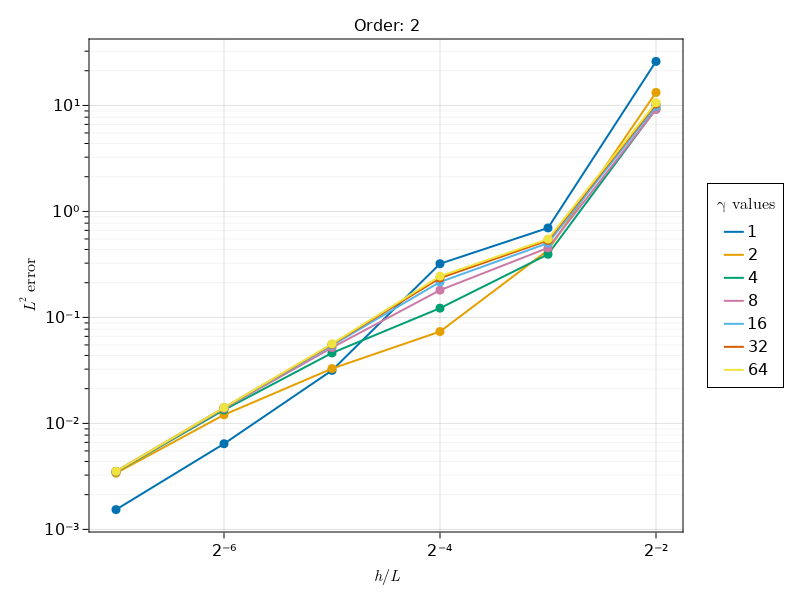
\includegraphics[scale=.25]{figures/convergence/L_1.0_m_7_r_3/gamma_analysis_order2.png}}
    \end{minipage}%
    \begin{minipage}{.5\linewidth}
    \centering
    \subfloat[]{\label{fig:ex1_gamma:b}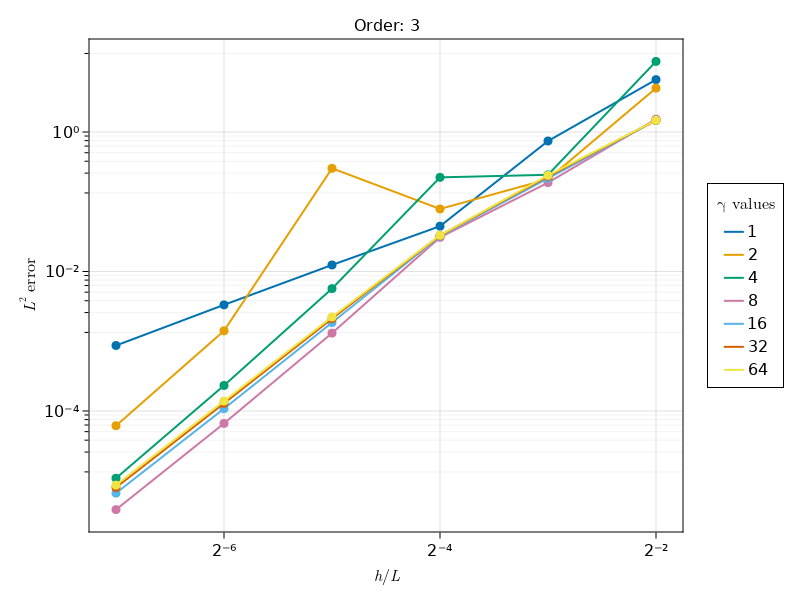
\includegraphics[scale=.25]{figures/convergence/L_1.0_m_7_r_3/gamma_analysis_order3.png}}
    \end{minipage}\par\medskip
    \centering
    \subfloat[]{\label{fig:ex1_gamma:c}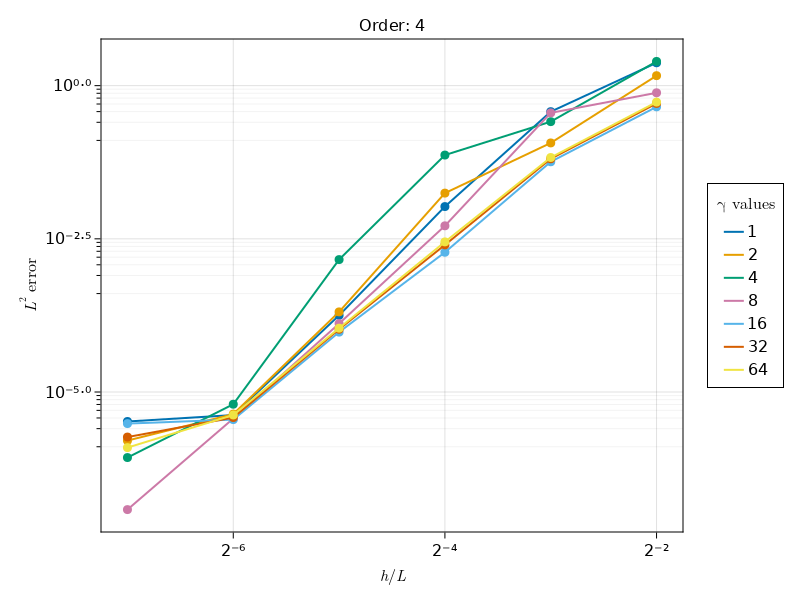
\includegraphics[scale=.25]{figures/convergence/L_1.0_m_7_r_3/gamma_analysis_order4.png}}
    \caption{ Convergence study for penalty parameters $\gamma$ with the model parameters $L=1$, $m=7$ and $r=3$. Figures \ref{fig:ex1_gamma:a}, \ref{fig:ex1_gamma:b} and \ref{fig:ex1_gamma:c} has respectively the order $k=2,3, 4$.  }
    \label{fig:ex1_gamma}
\end{figure}


\begin{figure}
    \centering
    \begin{minipage}{.5\linewidth}
    \centering
    \subfloat[]{\label{fig:ex1_conv:a}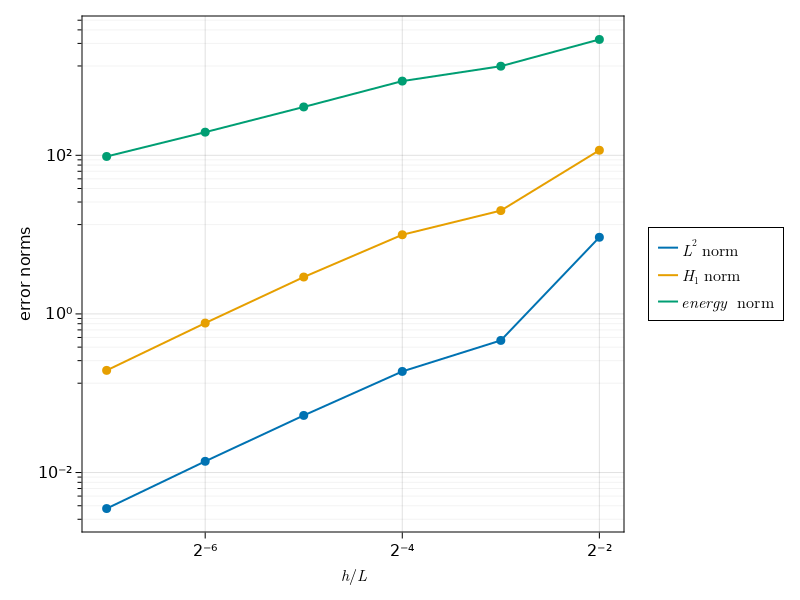
\includegraphics[scale=.25]{figures/convergence/L_1.0_m_7_r_3/conv_order_2_gamma_9.0.png}}
    \end{minipage}%
    \begin{minipage}{.5\linewidth}
    \centering
    \subfloat[]{\label{fig:ex1_conv:b}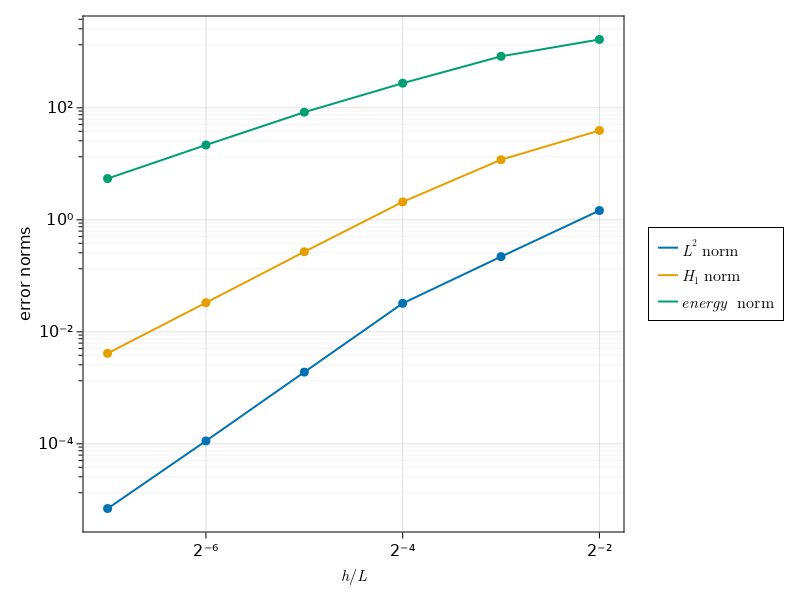
\includegraphics[scale=.25]{figures/convergence/L_1.0_m_7_r_3/conv_order_3_gamma_18.0.png}}
    \end{minipage}\par\medskip
    \centering
    \subfloat[]{\label{fig:ex1_conv:c}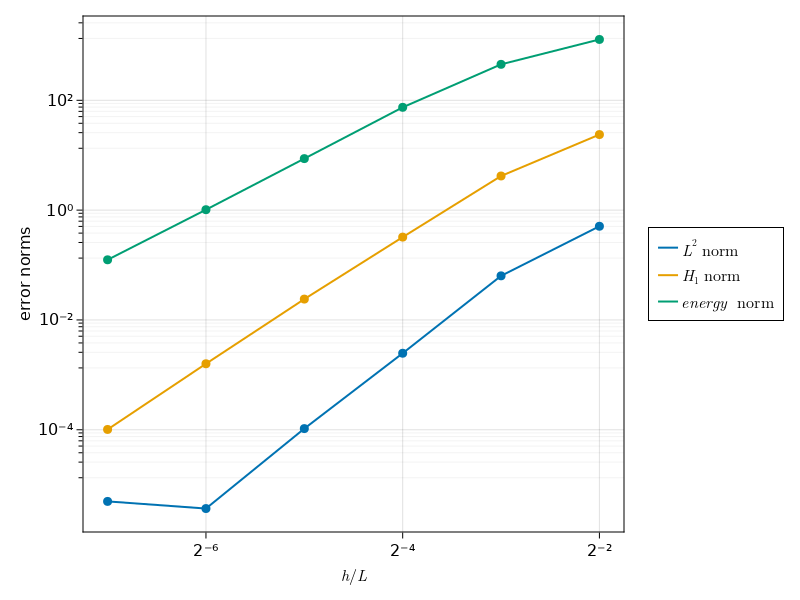
\includegraphics[scale=.25]{figures/convergence/L_1.0_m_7_r_3/conv_order_4_gamma_30.0.png}}
    \caption{ Convergence plots with model parameters $L=1$, $m=7$ and $r=3$ Figures \ref{fig:ex1_conv:a}, \ref{fig:ex1_conv:b} and \ref{fig:ex1_conv:c} has respectively the order $k=2,3, 4$ with penalty parameters $\gamma = 9,18,30 $.  }
    \label{fig:ex1_conv}
\end{figure}


% Gammas for L=1
\begin{table}
  \caption{\label{tab:ex1_order:a} Convergence table with the model parameters $L=1$, $m=7$ and $r=3$ with order $k=2$ using $ \gamma = 9$}
  \begin{tabular}{rrrrrrrr}
    \hline\hline
    $i$&\textbf{$h/{L} $} & \textbf{$L^2$ norm} & \textbf{EOC} & \textbf{$H_1$ norm} & \textbf{EOC} & \textbf{energy norm} & \textbf{EOC} \\\hline
    0&$\frac{1}{4}$ & 9.253E+00 &  & 1.158E+02 &  & 2.888E+03 &  \\
    1&$\frac{1}{8}$ & 4.632E-01 & 4.320E+00 & 2.008E+01 & 2.527E+00 & 1.328E+03 & 1.120E+00 \\
    2&$\frac{1}{16}$ & 1.883E-01 & 1.299E+00 & 9.954E+00 & 1.013E+00 & 8.620E+02 & 6.238E-01 \\
    3&$\frac{1}{32}$ & 5.250E-02 & 1.842E+00 & 2.918E+00 & 1.770E+00 & 4.070E+02 & 1.083E+00 \\
    4&$\frac{1}{64}$ & 1.385E-02 & 1.922E+00 & 7.665E-01 & 1.929E+00 & 1.957E+02 & 1.056E+00 \\
    5&$\frac{1}{128}$ & 3.515E-03 & 1.979E+00 & 1.941E-01 & 1.981E+00 & 9.665E+01 & 1.018E+00 \\\hline\hline
  \end{tabular}
% \end{table}
% \begin{table} .
  \caption{\label{tab:ex1_order:b} Convergence table with the model parameters $L=1$, $m=7$ and $r=3$ with order $k=3$ using $ \gamma = 18$ }
  \begin{tabular}{rrrrrrrr}
    \hline\hline
    $i$&\textbf{$h/{L} $} & \textbf{$L^2$ norm} & \textbf{EOC} & \textbf{$H_1$ norm} & \textbf{EOC} & \textbf{energy norm} & \textbf{EOC} \\\hline
    0&$\frac{1}{4}$ & 1.466E+00 &  & 3.942E+01 &  & 1.664E+03 &  \\
    1&$\frac{1}{8}$ & 2.203E-01 & 2.735E+00 & 1.184E+01 & 1.736E+00 & 8.318E+02 & 1.000E+00 \\
    2&$\frac{1}{16}$ & 3.231E-02 & 2.769E+00 & 2.092E+00 & 2.500E+00 & 2.758E+02 & 1.593E+00 \\
    3&$\frac{1}{32}$ & 1.910E-03 & 4.081E+00 & 2.690E-01 & 2.959E+00 & 8.364E+01 & 1.721E+00 \\
    4&$\frac{1}{64}$ & 1.127E-04 & 4.083E+00 & 3.316E-02 & 3.020E+00 & 2.171E+01 & 1.946E+00 \\
    5&$\frac{1}{128}$ & 6.988E-06 & 4.011E+00 & 4.131E-03 & 3.005E+00 & 5.461E+00 & 1.991E+00 \\\hline\hline
  \end{tabular}
% \end{table}

  \caption{\label{tab:ex1_order:c}Convergence table with the model parameters $L=1$, $m=7$ and $r=3$ with order $k=4$ using $ \gamma = 30$ }
% \begin{table}
  \begin{tabular}{rrrrrrrr}
    \hline\hline
    $i$&\textbf{$h/{L} $} & \textbf{$L^2$ norm} & \textbf{EOC} & \textbf{$H_1$ norm} & \textbf{EOC} & \textbf{energy norm} & \textbf{EOC} \\\hline
    0&$\frac{1}{4}$ & 5.083E-01 &  & 2.377E+01 &  & 1.282E+03 &  \\
    1&$\frac{1}{8}$ & 6.355E-02 & 3.000E+00 & 4.185E+00 & 2.506E+00 & 4.516E+02 & 1.505E+00 \\
    2&$\frac{1}{16}$ & 2.475E-03 & 4.682E+00 & 3.223E-01 & 3.699E+00 & 7.450E+01 & 2.600E+00 \\
    3&$\frac{1}{32}$ & 1.050E-04 & 4.559E+00 & 2.398E-02 & 3.749E+00 & 8.670E+00 & 3.103E+00 \\
    4&$\frac{1}{64}$ & 3.675E-06 & 4.837E+00 & 1.593E-03 & 3.912E+00 & 1.018E+00 & 3.090E+00 \\
    5&$\frac{1}{128}$ & 4.958E-06 & -4.319E-01 & 1.013E-04 & 3.974E+00 & 1.246E-01 & 3.031E+00 \\\hline\hline
  \end{tabular}
\end{table}

\newpage

\begin{figure}
    \centering
    \begin{minipage}{.5\linewidth}
    \centering
    \subfloat[]{\label{fig:ex2_gamma:a}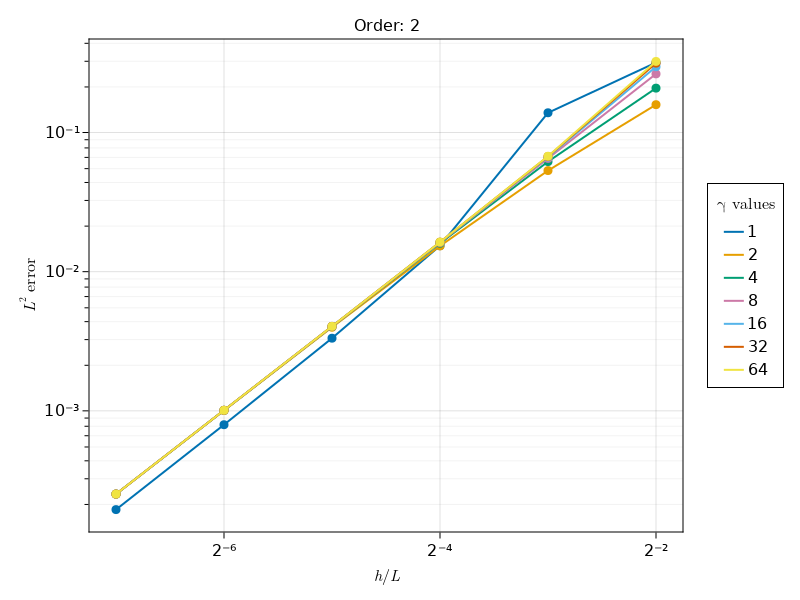
\includegraphics[scale=.25]{figures/convergence/L_6.28_m_1_r_1/gamma_analysis_order2.png}}
    \end{minipage}%
    \begin{minipage}{.5\linewidth}
    \centering
    \subfloat[]{\label{fig:ex2_gamma:b}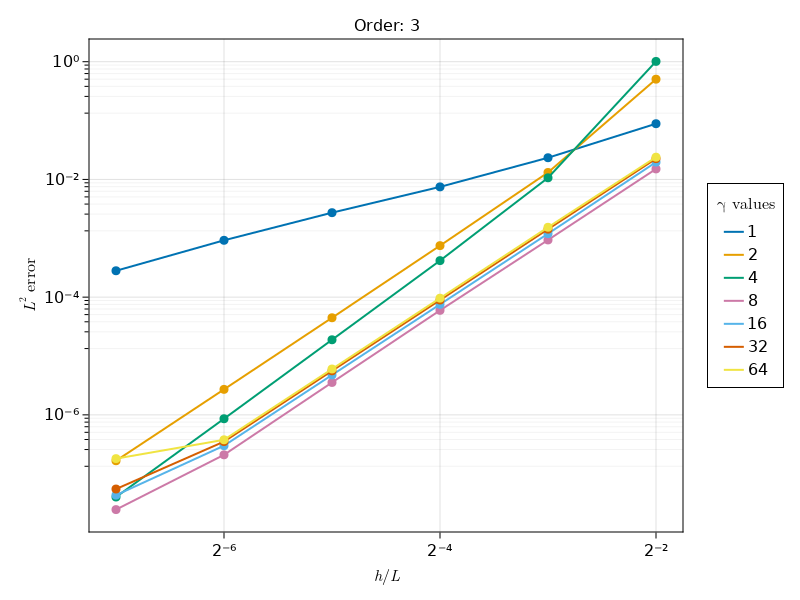
\includegraphics[scale=.25]{figures/convergence/L_6.28_m_1_r_1/gamma_analysis_order3.png}}
    \end{minipage}\par\medskip
    \centering
    \subfloat[]{\label{fig:ex2_gamma:c}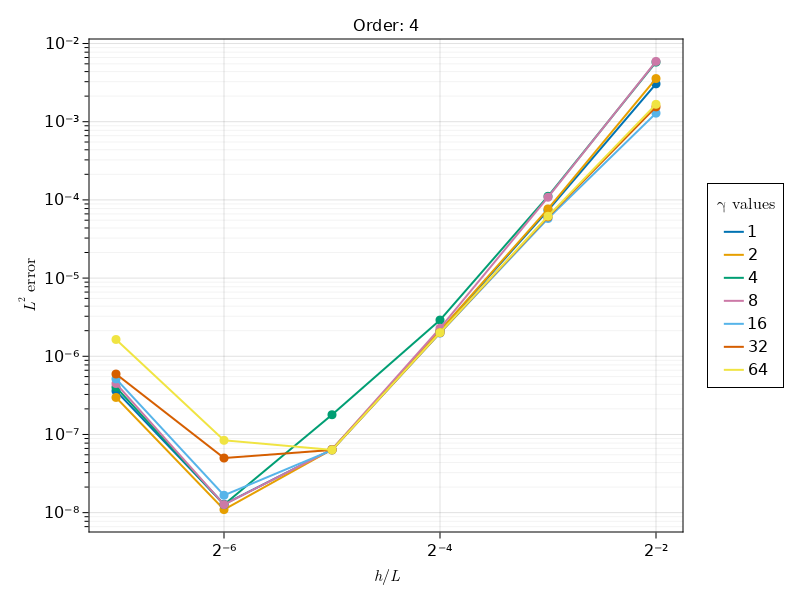
\includegraphics[scale=.25]{figures/convergence/L_6.28_m_1_r_1/gamma_analysis_order4.png}}
    \caption{ Convergence study for penalty parameters $\gamma$ with the model parameters $L=2\pi$, $m=1$ and $r=1$. Figures \ref{fig:ex1_gamma:a}, \ref{fig:ex1_gamma:b} and \ref{fig:ex1_gamma:c} has respectively the order $k=2,3, 4$.  }
    \label{fig:ex2_gamma}
\end{figure}

\begin{figure}
    \centering
    \begin{minipage}{.5\linewidth}
    \centering
    \subfloat[]{\label{fig:ex2_conv:a}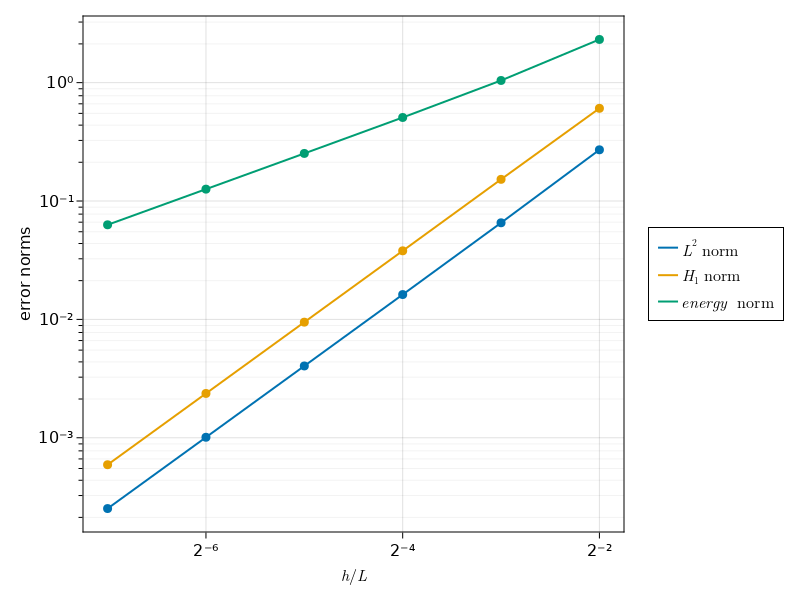
\includegraphics[scale=.25]{figures/convergence/L_6.28_m_1_r_1/conv_order_2_gamma_9.0.png}}
    \end{minipage}%
    \begin{minipage}{.5\linewidth}
    \centering
    \subfloat[]{\label{fig:ex2_conv:b}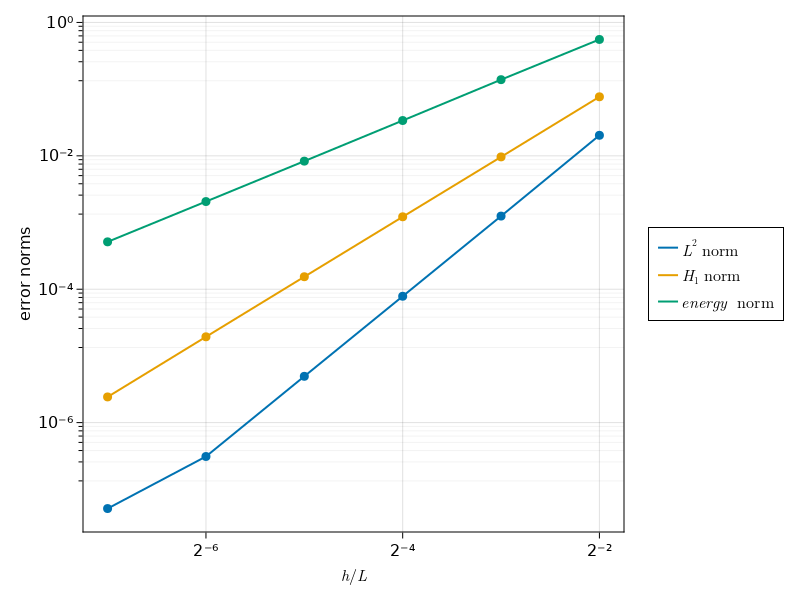
\includegraphics[scale=.25]{figures/convergence/L_6.28_m_1_r_1/conv_order_3_gamma_18.0.png}}
    \end{minipage}\par\medskip
    \centering
    \subfloat[]{\label{fig:ex2_conv:c}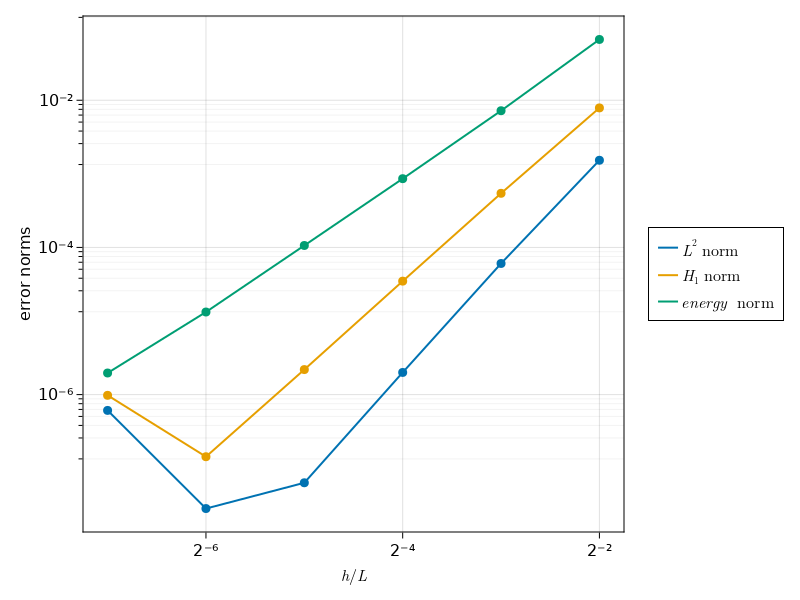
\includegraphics[scale=.25]{figures/convergence/L_6.28_m_1_r_1/conv_order_4_gamma_30.0.png}}
    \caption{ Convergence plots with model parameters $L=2\pi$, $m=1$ and $r=1$. Figures \ref{fig:ex2_conv:a}, \ref{fig:ex2_conv:b} and \ref{fig:ex2_conv:c} has respectively the order $k=2,3, 4$ with penalty parameters $\gamma = 9,18,30 $.  }
    \label{fig:ex2_conv}
\end{figure}



% Gammas for L=2pi
\begin{table}
  \caption{\label{tab:ex2_order:a} Convergence table with the model parameters $L=2\pi$, $m=1$ and $r=1$ with order $k=2$ using $ \gamma = 9$}
  \begin{tabular}{rrrrrrrr}
    \hline\hline
    $i$&\textbf{$h/{L} $} & \textbf{$L^2$ norm} & \textbf{EOC} & \textbf{$H_1$ norm} & \textbf{EOC} & \textbf{energy norm} & \textbf{EOC} \\\hline
    0&$\frac{1}{4}$ & 2.708E-01 &  & 6.068E-01 &  & 2.316E+00 &  \\
    1&$\frac{1}{8}$ & 6.547E-02 & 2.048E+00 & 1.524E-01 & 1.993E+00 & 1.043E+00 & 1.151E+00 \\
    2&$\frac{1}{16}$ & 1.621E-02 & 2.014E+00 & 3.796E-02 & 2.006E+00 & 5.078E-01 & 1.039E+00 \\
    3&$\frac{1}{32}$ & 4.041E-03 & 2.004E+00 & 9.475E-03 & 2.002E+00 & 2.523E-01 & 1.009E+00 \\
    4&$\frac{1}{64}$ & 1.010E-03 & 2.001E+00 & 2.367E-03 & 2.001E+00 & 1.260E-01 & 1.002E+00 \\
    5&$\frac{1}{128}$ & 2.524E-04 & 2.000E+00 & 5.918E-04 & 2.000E+00 & 6.296E-02 & 1.001E+00 \\\hline\hline
  \end{tabular}
% \end{table}

% \begin{table}
  \caption{\label{tab:ex2_order:b} Convergence table with the model parameters $L=2\pi$, $m=1$ and $r=1$ with order $k=3$ using $ \gamma = 18$}
  \begin{tabular}{rrrrrrrr}
    \hline\hline
    $i$&\textbf{$h/{L} $} & \textbf{$L^2$ norm} & \textbf{EOC} & \textbf{$H_1$ norm} & \textbf{EOC} & \textbf{energy norm} & \textbf{EOC} \\\hline
    0&$\frac{1}{4}$ & 2.032E-02 &  & 7.678E-02 &  & 5.558E-01 &  \\
    1&$\frac{1}{8}$ & 1.249E-03 & 4.024E+00 & 9.639E-03 & 2.994E+00 & 1.387E-01 & 2.003E+00 \\
    2&$\frac{1}{16}$ & 7.845E-05 & 3.993E+00 & 1.219E-03 & 2.983E+00 & 3.385E-02 & 2.035E+00 \\
    3&$\frac{1}{32}$ & 4.946E-06 & 3.987E+00 & 1.539E-04 & 2.986E+00 & 8.327E-03 & 2.023E+00 \\
    4&$\frac{1}{64}$ & 3.104E-07 & 3.994E+00 & 1.935E-05 & 2.992E+00 & 2.063E-03 & 2.013E+00 \\
    5&$\frac{1}{128}$ & 5.147E-08 & 2.592E+00 & 2.427E-06 & 2.995E+00 & 5.134E-04 & 2.007E+00 \\\hline\hline
  \end{tabular}
% \end{table}

% \begin{table}
  \caption{\label{tab:ex2_order:c} Convergence table with the model parameters $L=2\pi$, $m=1$ and $r=1$ with order $k=4$ using $ \gamma = 30$}
  \begin{tabular}{rrrrrrrr}
    \hline\hline
    $i$&\textbf{$h/{L} $} & \textbf{$L^2$ norm} & \textbf{EOC} & \textbf{$H_1$ norm} & \textbf{EOC} & \textbf{energy norm} & \textbf{EOC} \\\hline
    0&$\frac{1}{4}$ & 1.529E-03 &  & 7.869E-03 &  & 6.700E-02 &  \\
    1&$\frac{1}{8}$ & 6.050E-05 & 4.660E+00 & 5.437E-04 & 3.855E+00 & 7.205E-03 & 3.217E+00 \\
    2&$\frac{1}{16}$ & 2.000E-06 & 4.919E+00 & 3.482E-05 & 3.965E+00 & 8.594E-04 & 3.068E+00 \\
    3&$\frac{1}{32}$ & 6.335E-08 & 4.980E+00 & 2.189E-06 & 3.992E+00 & 1.063E-04 & 3.016E+00 \\
    4&$\frac{1}{64}$ & 2.828E-08 & 1.164E+00 & 1.432E-07 & 3.934E+00 & 1.325E-05 & 3.003E+00 \\
    5&$\frac{1}{128}$ & 6.097E-07 & -4.430E+00 & 9.776E-07 & -2.772E+00 & 1.965E-06 & 2.753E+00 \\\hline\hline
  \end{tabular}
\end{table}



    % 
\newpage
\section{Cahn Hilliard Equation on a Closed Membrane}%
\label{sec:cahn_hilliard_equation}


Let $c_0$ and $c_1$  indicate the concentration profile of the substances in a a $2$ -phase system such
that $c_0 \left( \mathbf{x},t \right): \Omega  \times \left[ 0, \infty \right] \to \left[ 0,1 \right]$ and
similarly $c_1 \left( \mathbf{x},t \right): \Omega \times \left[ 0, \infty \right] \to \left[ 0,1 \right]$, where
$\mathbf{x} $ is a element of some surface $\Omega $ and $t$ is time.
However, in the $2$ phase problem will we will restrict ourself so that $c_0\left( t,\mathbf{x} \right) + c_1\left( t,
\mathbf{x} \right) = 1$ at any $\mathbf{x} $ at time $t$. A property of the restriction is that we now can express
$c_0$ using $c_1$, with no loss of information. Hence, let us now define $c = c_0$ so $c \left( \mathbf{x},t \right):
\Omega  \times \left[ 0, \infty \right] \to \left[ 0,1 \right]$. It has been shown that $2$ phase system if
thermodynamically unstabl can be evolve
into a phase seperation
described by a evolutional differential equation \cite{cahnhilliard1957} using a model based on chemical energy of the
substances. However, further development has been done \cite{yushutin19} to solve this equation on surfaces. Now assume
model that we want to describe is a phase-seperation on a closed membrane surface $\Gamma $, so that $c \left( \mathbf{x},t \right):
\Gamma \times \left[ 0, T \right] \to \left[ 0,1 \right]$. Then is the surface Cahn Hilliard equation described such that

\begin{equation}
    \label{eq:cahn1}
\rho \frac{\partial c}{\partial  t}  - \nabla_{\Gamma } \left( M \nabla _{\Gamma } \left( f_{0}'  - \varepsilon ^2
        \nabla^2
_{\Gamma } c \right) \right) = 0  \quad \text{on } \Gamma
.\end{equation}

We define here the tangential gradient operator to be $\nabla _{\Gamma } c = \nabla c - \left( \mathbf{n} \nabla c
\right)\mathbf{n} $ applied on the surface $\Gamma $ restricted to $\mathbf{n} \cdot \nabla _{\Gamma } c = 0$.

Lets define $\varepsilon $ to be the size of the layer between the substances $c_{1}$ and $c_{2}$. The density $\rho $ is
simply defined such that $\rho = \frac{m}{S_{\Gamma }}$ is a constant based on the total mass divaded by the total
surface area of $\Gamma $.
Here is the mobility $M$ often derived such that is is dependent on $c$ and is crucial for the result during a possible
coarsering event \cite{yushutin19}.  However, the free energy per unit surface
$f_{0} = f_{0}\left( c \right)$ is derived based on the thermodynamical model and should according to \cite{yushutin19} be nonconvex and
nonlinear.

A important observation is that equation \eqref{eq:cahn1} is a fourth order equation which makes it more challenging to
solve using conventional FEM methods. This clear when writing the equation on the equivalent weak form and second order
equations arise.


\newpage

    \newpage
\section{Appendix}%
\label{sec:appendix}

\subsection{The Space $L^{2} \left( \Omega  \right)$ }%
\label{sub:l_2_space}

Using the definition from \cite{manzoni2021optimal} and we let $\Omega $ be a an open set in $\mathbb{R} ^{d}$ and $p \in \mathbb{R} $  such that $p \ge 1$. Then we denote
$L^{p}\left( \Omega  \right) $ to be the set of measurable function $u: \Omega \to \mathbb{R} $ such that  it is equipped
in a finite Banach space \[
\|u\|_{L^{p}\left( \Omega  \right)}^{} = \left( \int_{\Omega }^{} \left\lvert u \right\rvert ^{p}
\right)^{\frac{1}{p}}.
\]

Now let $u,v: \Omega  \to \mathbb{R} $. Then is $L^{2}\left( \Omega  \right)$ a Hilbert space when the inner product is
finite such that this exists \[
\left( u,v \right)_{L^{p}\left( \Omega   \right)} = \int_{\Omega }^{} uv  .
\]
If the integral is finite do we say that $u,v \in L^{p}\left( \Omega  \right)$.



\subsection{The Space $H^{m} \left( \Omega  \right)$, $m>1$  }%
\label{sub:h_2_space}

Again using the definition from \cite{manzoni2021optimal}. Let $\alpha=\left( \alpha _{1}, \ldots, \alpha _{d} \right),
\quad \alpha \ge  0$, such that $\left\lvert \alpha  \right\rvert = \sum_{i=1}^{d} \alpha _{i} $. Now we define
the space \[
H^{m}\left( \Omega  \right) = \left\{ u \in L^2\left( \Omega  \right) : D^{\alpha } u \in L^2\left( \Omega  \right)\quad
\forall \alpha : \left\lvert \alpha  \right\rvert  \le  m \right\}.
\]


Suppose that $u,v$ is measurable functions. We can now define $u \in H^{m}\left( \Omega  \right)$  the Banach space is
finite . \[
\|u\|_{H^{m}\left( \Omega  \right)}^{} = \left( \|u\|_{L^2\left( \Omega  \right)}^{}  + \sum_{k=1}^{m}
\left\lvert u \right\rvert ^2 _{H^{k}\left( \Omega  \right)} \right), \quad \left\lvert u \right\rvert_ { H^{k} \left(
\Omega  \right) }  = \sqrt{\sum_{\left\lvert \alpha  \right\rvert = k  }^{} \| D^{\alpha }u \|_{L^2\left( \Omega  \right)
}^{ 2 } }
 \]

 Similarly for the finite Hilbert space \[
 \left( u,v \right)_{ H^{m} \left( \Omega  \right)}  = \sum_{\left\lvert \alpha  \right\rvert  \le  m}^{}  \int_{\Omega }^{}
 D^{\alpha } u D^{\alpha } v
 \]









    \newpage
    \printbibliography

\end{document}
